\documentclass[10pt,conference,twocolumn]{IEEEtran}
\IEEEoverridecommandlockouts
\usepackage{cite}
\usepackage{amsmath,amssymb,amsfonts}
\usepackage{graphicx}
\usepackage{booktabs}
\usepackage{stfloats}
\usepackage{hyperref}

\hypersetup{
    colorlinks=true,
    linkcolor=blue,
    citecolor=blue,
    urlcolor=blue
}

\begin{document}

\title{Validade Temporal e Supersessão de Fatos em Memória Associativa Hebbiana para Agentes Baseados em LLM}

\author{\IEEEauthorblockN{Filipe Augusto de Ataíde Barbosa}
\IEEEauthorblockA{\textit{Centro de Informática (CIn) --- Universidade Federal de Pernambuco (UFPE)}\\
Recife, Brasil --- faab@cin.ufpe.br}
}

\maketitle

\begin{abstract}
Arquiteturas de memória associativa baseadas em plasticidade hebbiana, como o \textit{HeLa-Mem} (ACL 2026), destacam-se na recuperação de múltiplos saltos (\textit{multi-hop}), mas tratam fatos extraídos como estáticos, confundindo a recência do registro com a validade temporal do fato. Este trabalho apresenta a avaliação experimental controlada (Baseline A vs. Proposta B) no benchmark \textit{LongMemEval-S} (500 instâncias). A replicação estrita da Baseline A atingiu 61,20\% de acurácia global (306/500), revelando que 43,8\% das falhas concentram-se em raciocínio temporal e atualização de conhecimento devido à recuperação de fatos obsoletos e à omissão de timestamps de sessão na memória semântica. Para superar esse gargalo, implementou-se a extensão \texttt{TemporalKnowledgeMemory} acoplada ao \texttt{ValidityAwareRetriever}, introduzindo janelas explícitas de validade $[t_{start}, t_{end}]$, transições não-destrutivas de supersessão (\texttt{SUPERSEDES}) e ponderação por pertinência temporal $\mathcal{V}(f_i, t_{query})$. Nos 500 itens oficiais, a Proposta B elevou a acurácia global para \textbf{65,60\% (328/500)}, obtendo um ganho líquido de \textbf{+4,40 p.p. (+22 instâncias, $p = 0,0115$ no teste exato de McNemar)} e superando a meta oficial reportada no artigo da ACL 2026 (65,40\%). Os maiores avanços ocorreram justamente nas categorias-alvo: \textit{Knowledge Update} (\textbf{83,33\% vs. 73,08\%, +10,26 p.p.}), \textit{Single-Session Preference} (\textbf{+20,00 p.p.}), \textit{Single-Session Assistant} (\textbf{+5,36 p.p.}), \textit{Temporal Reasoning} (\textbf{55,64\% vs. 51,88\%, +3,76 p.p.}) e \textit{Multi-Session} (\textbf{+2,26 p.p.}).
\end{abstract}

\begin{IEEEkeywords}
Memória para Agentes, Aprendizado Hebbiano, Validade Temporal, Supersessão Factual, LongMemEval-S.
\end{IEEEkeywords}

\begin{figure*}[!t]
\centering
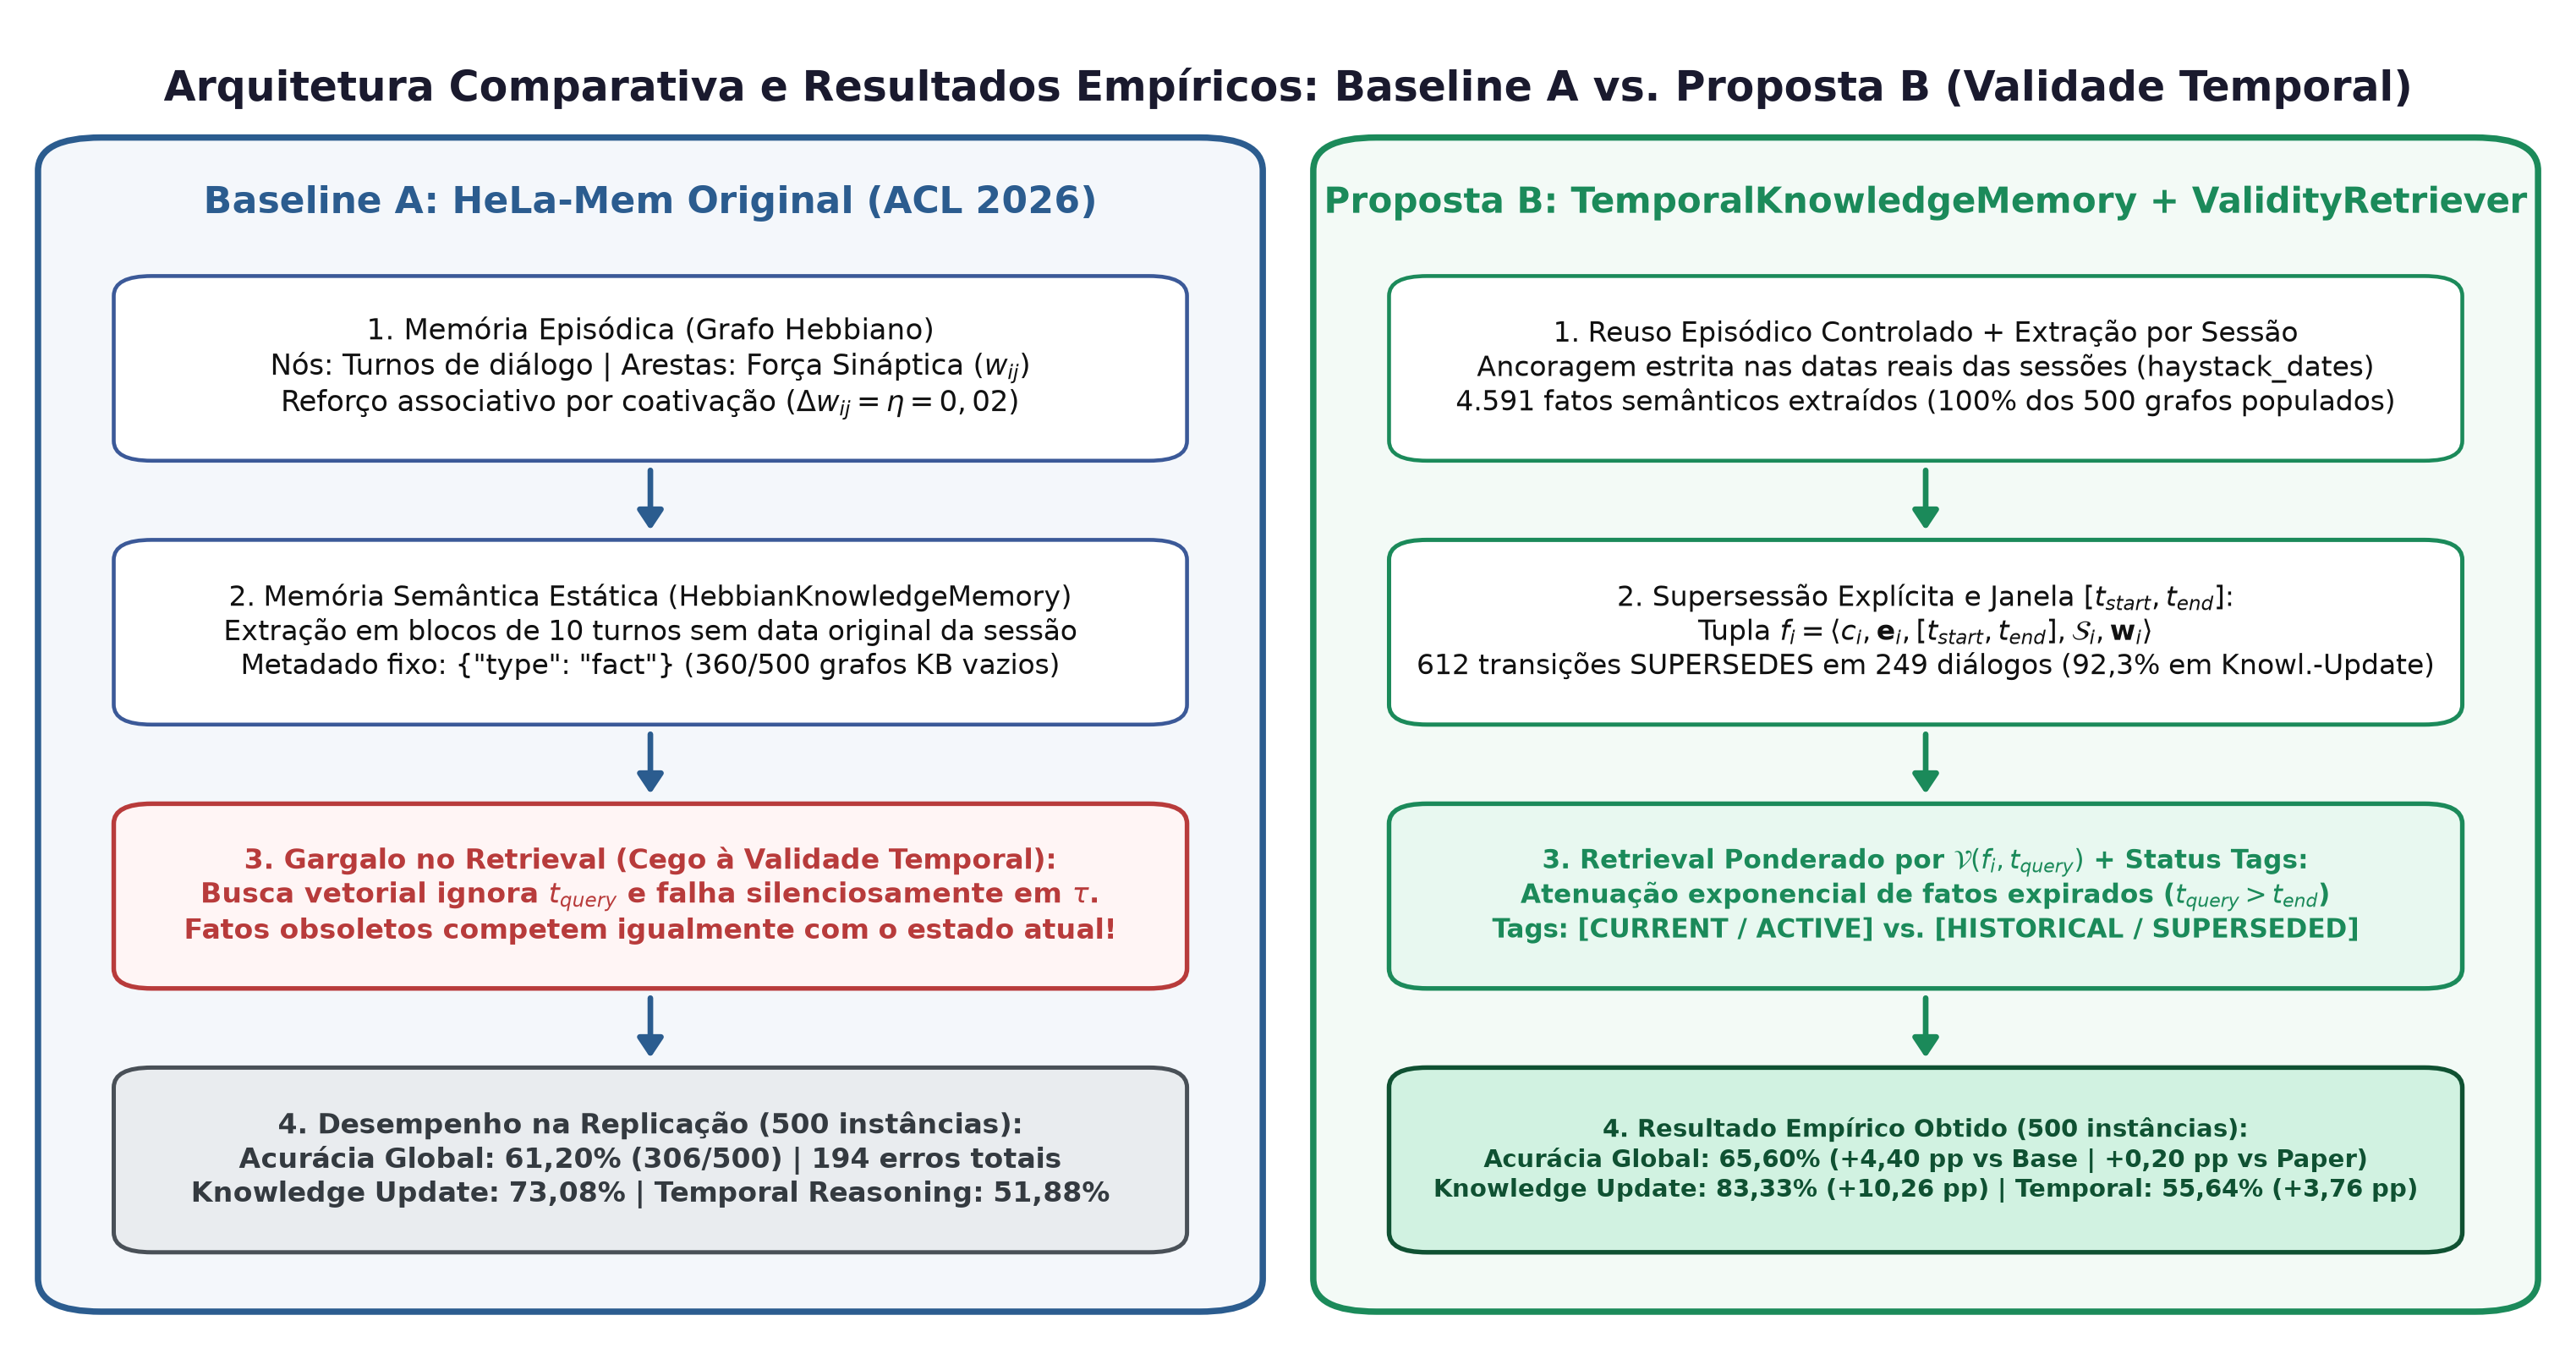
\includegraphics[width=\textwidth]{figures/fig1_arquitetura_proposta.png}
\caption{Contraste arquitetural e resultados consolidados nos 500 itens do \textit{LongMemEval-S}: (Esquerda) Baseline A (\textit{HeLa-Mem} original) com fatos semânticos atemporais, extração em blocos que deixou 360/500 grafos semânticos vazios e busca cega a $t_{query}$ (61,20\% global); (Direita) Proposta B com extração ancorada na sessão, janelas de validade $[t_{start}, t_{end}]$, 612 arestas \texttt{SUPERSEDES} e retrieval ponderado por pertinência temporal $\mathcal{V}(f_i, t_{query})$ (65,60\% global, +10,26 p.p. em \textit{Knowledge Update}).}
\label{fig:arquitetura}
\end{figure*}

% =========================================================================
% SEÇÃO I: INTRODUÇÃO E SOLUÇÃO PROPOSTA
% =========================================================================
\section{Solução Proposta}

\subsection{Diagnóstico: Plasticidade Associativa vs. Validade Temporal}
No \textit{HeLa-Mem}~\cite{helamem2026}, conexões entre nós episódicos coativados são fortalecidas por aprendizado hebbiano ($\Delta w_{ij} = \eta$), favorecendo a recuperação associativa por ativação espalhada (\textit{spreading activation}). Contudo, a auditoria empírica do código oficial (\texttt{HebbianKnowledgeMemory}) revelou três limitações estruturais no tratamento da evolução factual:
\begin{enumerate}
    \item \textbf{Atemporalidade Semântica}: Fatos consolidados são armazenados apenas com o metadado estático \texttt{\{"type": "fact"\}} e recebem o horário de execução do script (\texttt{get\_timestamp()}) em vez da data real da sessão do diálogo (\texttt{haystack\_dates}).
    \item \textbf{Competição entre Fatos Conflitantes}: Quando um atributo do usuário muda ao longo do tempo (ex.: mudança de endereço, hábito ou status), o fato antigo e o novo coexistem com pesos positivos e competem igualmente na busca por similaridade de cosseno.
    \item \textbf{Neutralização Silenciosa do Decaimento e Omissão de $t_{query}$}: Em \texttt{hebbian\_retriever.py}, a chamada \texttt{compute\_time\_decay(node["timestamp"], current\_time)} passa uma string de data no lugar da constante escalar $\tau$, caindo silenciosamente em \texttt{except: return 1.0}. Ademais, a data da pergunta (\texttt{question\_date}) é injetada apenas no prompt final de geração, sendo ignorada durante a etapa de \textit{retrieval}.
\end{enumerate}

\subsection{Formalização e Mecanismo de Supersessão}
Inspirada em grafos de conhecimento temporais~\cite{zep2025}, a extensão implementada (\texttt{TemporalKnowledgeMemory}) preserva intacto o grafo episódico hebbiano e reformula a memória semântica (Fig.~\ref{fig:arquitetura}). Cada fato consolidado $f_i \in \mathcal{F}$ passa a ser representado pela 5-upla:
\begin{equation}
f_i = \langle c_i, \mathbf{e}_i, [t_{start}^{(i)}, t_{end}^{(i)}], \mathcal{S}_i, \mathbf{w}_i \rangle
\end{equation}
onde $c_i$ é o conteúdo proposicional do fato, $\mathbf{e}_i \in \mathbb{R}^d$ o vetor de embedding normalizado, $[t_{start}^{(i)}, t_{end}^{(i)}]$ o intervalo explícito de validade ancorado no timestamp original da sessão ($t_{end}^{(i)} = \infty$ enquanto ativo), $\mathcal{S}_i$ o ponteiro bidirecional de supersessão (\texttt{superseded\_by} / \texttt{supersedes}) e $\mathbf{w}_i$ o vetor de pesos sinápticos hebbianos.

Ao extrair um novo fato $f_{new}$ de uma sessão ocorrida em $t_{event}$, o sistema filtra candidatos ativos de sessões anteriores ($\mathcal{F}_{active} = \{f_cand \mid t_{end}^{(cand)} = \infty \land t_{start}^{(cand)} \neq t_{event}\}$) cuja similaridade semântica $\mathbf{e}_{new}^\top \mathbf{e}_{cand} \ge \theta_{sup}$ ($\theta_{sup} = 0,35$). A restrição $t_{start}^{(cand)} \neq t_{event}$ impede falsos positivos de supersessão entre fatos complementares extraídos de uma mesma sessão. Os candidatos do topo são submetidos a um classificador de consistência factual em três estados:
\begin{itemize}
    \item \textbf{UNRELATED}: fatos sobre entidades ou tópicos independentes; ambos permanecem ativos ($t_{end} = \infty$).
    \item \textbf{EXTENDS}: $f_{new}$ detalha ou complementa $f_{cand}$ sem contradição; reforça-se a associação hebbiana $w(f_{cand}, f_{new}) \leftarrow w(f_{cand}, f_{new}) + \eta$.
    \item \textbf{SUPERSEDES}: $f_{new}$ atualiza, substitui ou altera o estado/localização/preferência de $f_{cand}$, encerrando sua vigência de forma não-destrutiva:
    \begin{align}
    t_{end}^{(cand)} &\leftarrow t_{event}, \quad \mathcal{S}_{cand} \leftarrow f_{new}, \nonumber \\
    [t_{start}^{(new)}, t_{end}^{(new)}] &\leftarrow [t_{event}, \infty)
    \end{align}
    Adicionalmente, cria-se uma aresta direcionada de transição com peso forte ($w = 0,8$) entre $f_{cand}$ e $f_{new}$, permitindo recuperar a linhagem histórica quando a pergunta exigir estados passados.
\end{itemize}

\begin{figure*}[!t]
\centering
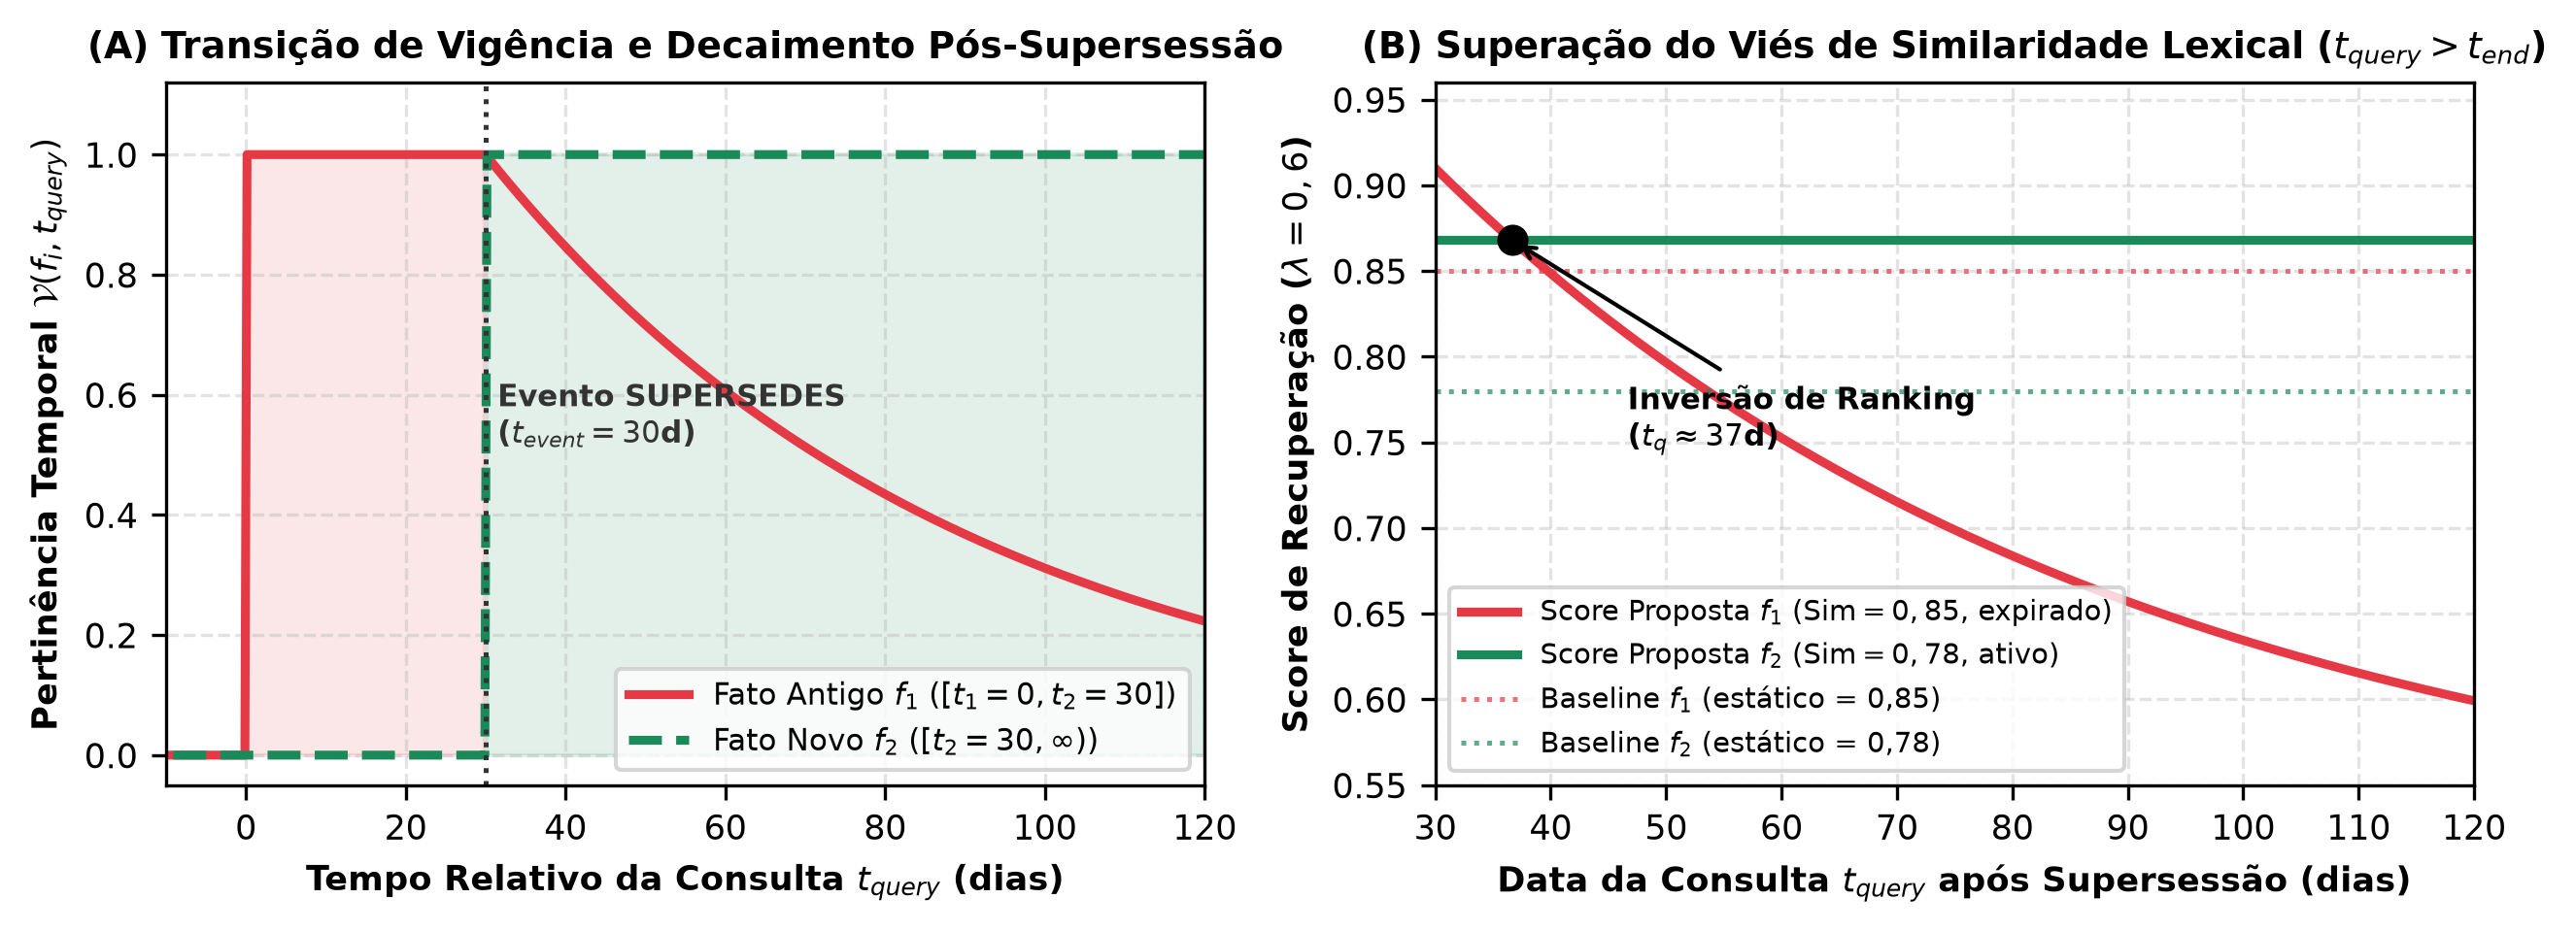
\includegraphics[width=0.92\textwidth]{figures/fig5_decaimento_pertinencia.png}
\caption{Modelagem matemática da pertinência temporal $\mathcal{V}(f_i, t_{query})$: (A) Fechamento da janela de vigência de $f_1$ no evento de supersessão ($t_{event}=30$d) e decaimento exponencial suave ($\tau_{decay}=60$d); (B) Inversão de ranking no \textit{retrieval} ($\lambda=0,6$), permitindo que o fato atualizado $f_2$ ($\text{Sim}=0,78$) supere o fato obsoleto $f_1$ ($\text{Sim}=0,85$) após o ponto de cruzamento.}
\label{fig:decaimento}
\end{figure*}

\subsection{Retrieval Ponderado por Pertinência Temporal e Grounding}
No momento da consulta $Q$ formulada em $t_{query}$, o módulo \texttt{ValidityAwareRetriever} calcula a pertinência temporal $\mathcal{V}(f_i, t_{query})$ de cada fato semântico:
\begin{equation}
\mathcal{V}(f_i, t_{query}) = 
\begin{cases}
1.0, & \text{se } t_{start}^{(i)} \le t_{query} \le t_{end}^{(i)} \\
\exp\left(-\frac{|t_{query} - t_{end}^{(i)}|}{\tau_{decay}}\right), & \text{se } t_{query} > t_{end}^{(i)} \text{ (expirado)} \\
0.0, & \text{se } t_{query} < t_{start}^{(i)} \text{ (futuro)}
\end{cases}
\end{equation}
O score base combina similaridade semântica reescalada $\widetilde{\text{Sim}}(\mathbf{e}_i, \mathbf{e}_Q) = (\mathbf{e}_i^\top \mathbf{e}_Q + 1)/2 \in [0,1]$ e pertinência temporal ($\lambda = 0,6$, $\tau_{decay} = 60\text{ dias}$), propagando-se em seguida pelas arestas hebbianas:
\begin{equation}
\text{Score}(f_i, Q, t_{query}) = \lambda \cdot \widetilde{\text{Sim}}(\mathbf{e}_i, \mathbf{e}_Q) + (1-\lambda) \cdot \mathcal{V}(f_i, t_{query}) + \text{Spread}(f_i)
\end{equation}
Conforme demonstrado na Fig.~\ref{fig:decaimento}, essa formulação resolve o viés de similaridade lexical: mesmo quando um fato obsoleto $f_1$ possui maior sobreposição de palavras com a pergunta ($\widetilde{\text{Sim}} = 0,85$) do que o fato atualizado $f_2$ ($\widetilde{\text{Sim}} = 0,78$), a atenuação de $\mathcal{V}(f_1, t_{query})$ para $t_{query} > t_{end}^{(1)}$ inverte o ranking em favor do estado vigente, sem zerar abruptamente o fato antigo caso a pergunta consulte o passado. Por fim, os fatos recuperados são formatados no bloco \texttt{<KNOWLEDGE BASE>} com tags explícitas de estado: \texttt{[CURRENT / ACTIVE (Valid since: $t_{start}$)]} ou \texttt{[HISTORICAL / SUPERSEDED (Valid: $t_{start}$ to $t_{end}$)]}.

% =========================================================================
% SEÇÃO II: PROTOCOLO EXPERIMENTAL CONTROLADO (A vs. B)
% =========================================================================
\section{Protocolo Experimental Controlado (A vs. B)}

Para garantir rigor causal e isolar estritamente o efeito da Memória Semântica Temporal sobre o desempenho do agente, adotou-se um desenho experimental pareado A/B sobre a totalidade do benchmark \textbf{LongMemEval-S}~\cite{longmemeval2025} (500 instâncias distribuídas em 6 categorias de raciocínio de longo prazo):
\begin{itemize}
    \item \textbf{Controle Estrito da Memória Episódica}: A Proposta B reutiliza exatamente os mesmos 500 grafos episódicos (\texttt{<id>\_hebbian.json}) gerados pela Baseline A (\texttt{--reuse\_episodic\_dir}). Dessa forma, os nós episódicos, pesos sinápticos $w_{ij}$ e os top-15 trechos de diálogo recuperados são idênticos entre A e B, eliminando variância estocástica na camada episódica.
    \item \textbf{Correção da Extração por Sessão}: Na Baseline A, o buffer de extração a cada 10 turnos misturava datas distintas e deixou 360 dos 500 grafos semânticos vazios. Na Proposta B, os turnos são agrupados por sessão (\texttt{extract\_session\_turns}), preservando o timestamp exato de cada sessão e populando 100\% dos 500 grafos semânticos com um total de \textbf{4.591 fatos} (média de 9,18 fatos/item).
    \item \textbf{Modelos e Hiperparâmetros}: Utilizou-se o mesmo LLM de extração, geração e avaliação LLM-as-a-Judge (\texttt{gpt-4o-mini}), embeddings densos de 384 dimensões (\texttt{all-MiniLM-L6-v2}), $\text{top\_k}=15$ (episódico), $\text{semantic\_top\_k}=5$, $\alpha=0,1$, $\eta=0,02$, $\lambda=0,6$, $\theta_{sup}=0,35$ e $\tau_{decay}=60$ dias.
\end{itemize}

% =========================================================================
% SEÇÃO III: RESULTADOS E ANÁLISE QUANTITATIVA
% =========================================================================
\section{Resultados e Análise Quantitativa}

\subsection{Evolução Global e Desempenho por Categoria}
A Tabela~\ref{tab:ab_results} e a Fig.~\ref{fig:baseline_vs_paper} consolidam a evolução da acurácia entre o artigo original da ACL 2026~\cite{helamem2026}, a nossa replicação da Baseline A e a Proposta B nos 500 itens do \textit{LongMemEval-S}.

\begin{table*}[!t]
\caption{Comparação Quantitativa Completa no LongMemEval-S (500 Instâncias): Meta Oficial (ACL 2026), Replicação da Baseline A e Proposta B (Validade Temporal), incluindo Transições Pareadas e Estatísticas Estruturais do Grafo Semântico.}
\label{tab:ab_results}
\centering
\footnotesize
\setlength{\tabcolsep}{5.2pt}
\begin{tabular}{lccccccccc}
\toprule
\textbf{Categoria} & \textbf{Total} & \textbf{Paper ACL'26} & \textbf{Baseline A} & \textbf{Proposta B} & $\mathbf{\Delta (B - A)}$ & \textbf{Ganhos} & \textbf{Regr.} & \textbf{Saldo} & \textbf{Diálogos c/ Sup.} \\
\textbf{(\texttt{question\_type})} & \textbf{($N$)} & \textbf{(\%)} & \textbf{Acertos (\%)} & \textbf{Acertos (\%)} & \textbf{(p.p.)} & \textbf{($0 \to 1$)} & \textbf{($1 \to 0$)} & \textbf{Líquido} & \textbf{(Fatos Subst. \%)} \\
\midrule
\texttt{knowledge-update} & 78 & 78,21\% & 57 (73,08\%) & \textbf{65 (83,33\%)} & \textbf{+10,26} & +11 & -3 & \textbf{+8} & 92,3\% (20,41\%) \\
\texttt{temporal-reasoning} & 133 & 50,38\% & 69 (51,88\%) & \textbf{74 (55,64\%)} & \textbf{+3,76} & +15 & -10 & \textbf{+5} & 54,1\% (13,02\%) \\
\texttt{multi-session} & 133 & 57,14\% & 62 (46,62\%) & \textbf{65 (48,87\%)} & \textbf{+2,26} & +14 & -11 & \textbf{+3} & 78,9\% (15,70\%) \\
\texttt{single-session-preference} & 30 & ---$^\dagger$ & 8 (26,67\%) & \textbf{14 (46,67\%)} & \textbf{+20,00} & +8 & -2 & \textbf{+6} & 0,0\% (0,00\%) \\
\texttt{single-session-assistant} & 56 & ---$^\dagger$ & 49 (87,50\%) & \textbf{52 (92,86\%)} & \textbf{+5,36} & +3 & 0 & \textbf{+3} & 0,0\% (0,00\%) \\
\texttt{single-session-user} & 70 & 78,85\%$^\dagger$ & \textbf{61 (87,14\%)} & 58 (82,86\%) & -4,29 & +3 & -6 & -3 & 0,0\% (0,00\%) \\
\midrule
\textbf{OVERALL (Global)} & \textbf{500} & \textbf{65,40\%} & \textbf{306 (61,20\%)} & \textbf{328 (65,60\%)} & \textbf{+4,40} & \textbf{+54} & \textbf{-32} & \textbf{+22} & \textbf{49,8\% (13,33\%)} \\
\bottomrule
\multicolumn{10}{l}{\scriptsize $^\dagger$No artigo original da ACL 2026, as categorias de sessão única são reportadas agregadas sob \textit{Single-Session} com 78,85\% (na Proposta B, a média ponderada de sessão única é 79,49\%).}
\end{tabular}
\end{table*}

\begin{figure}[!t]
\centering
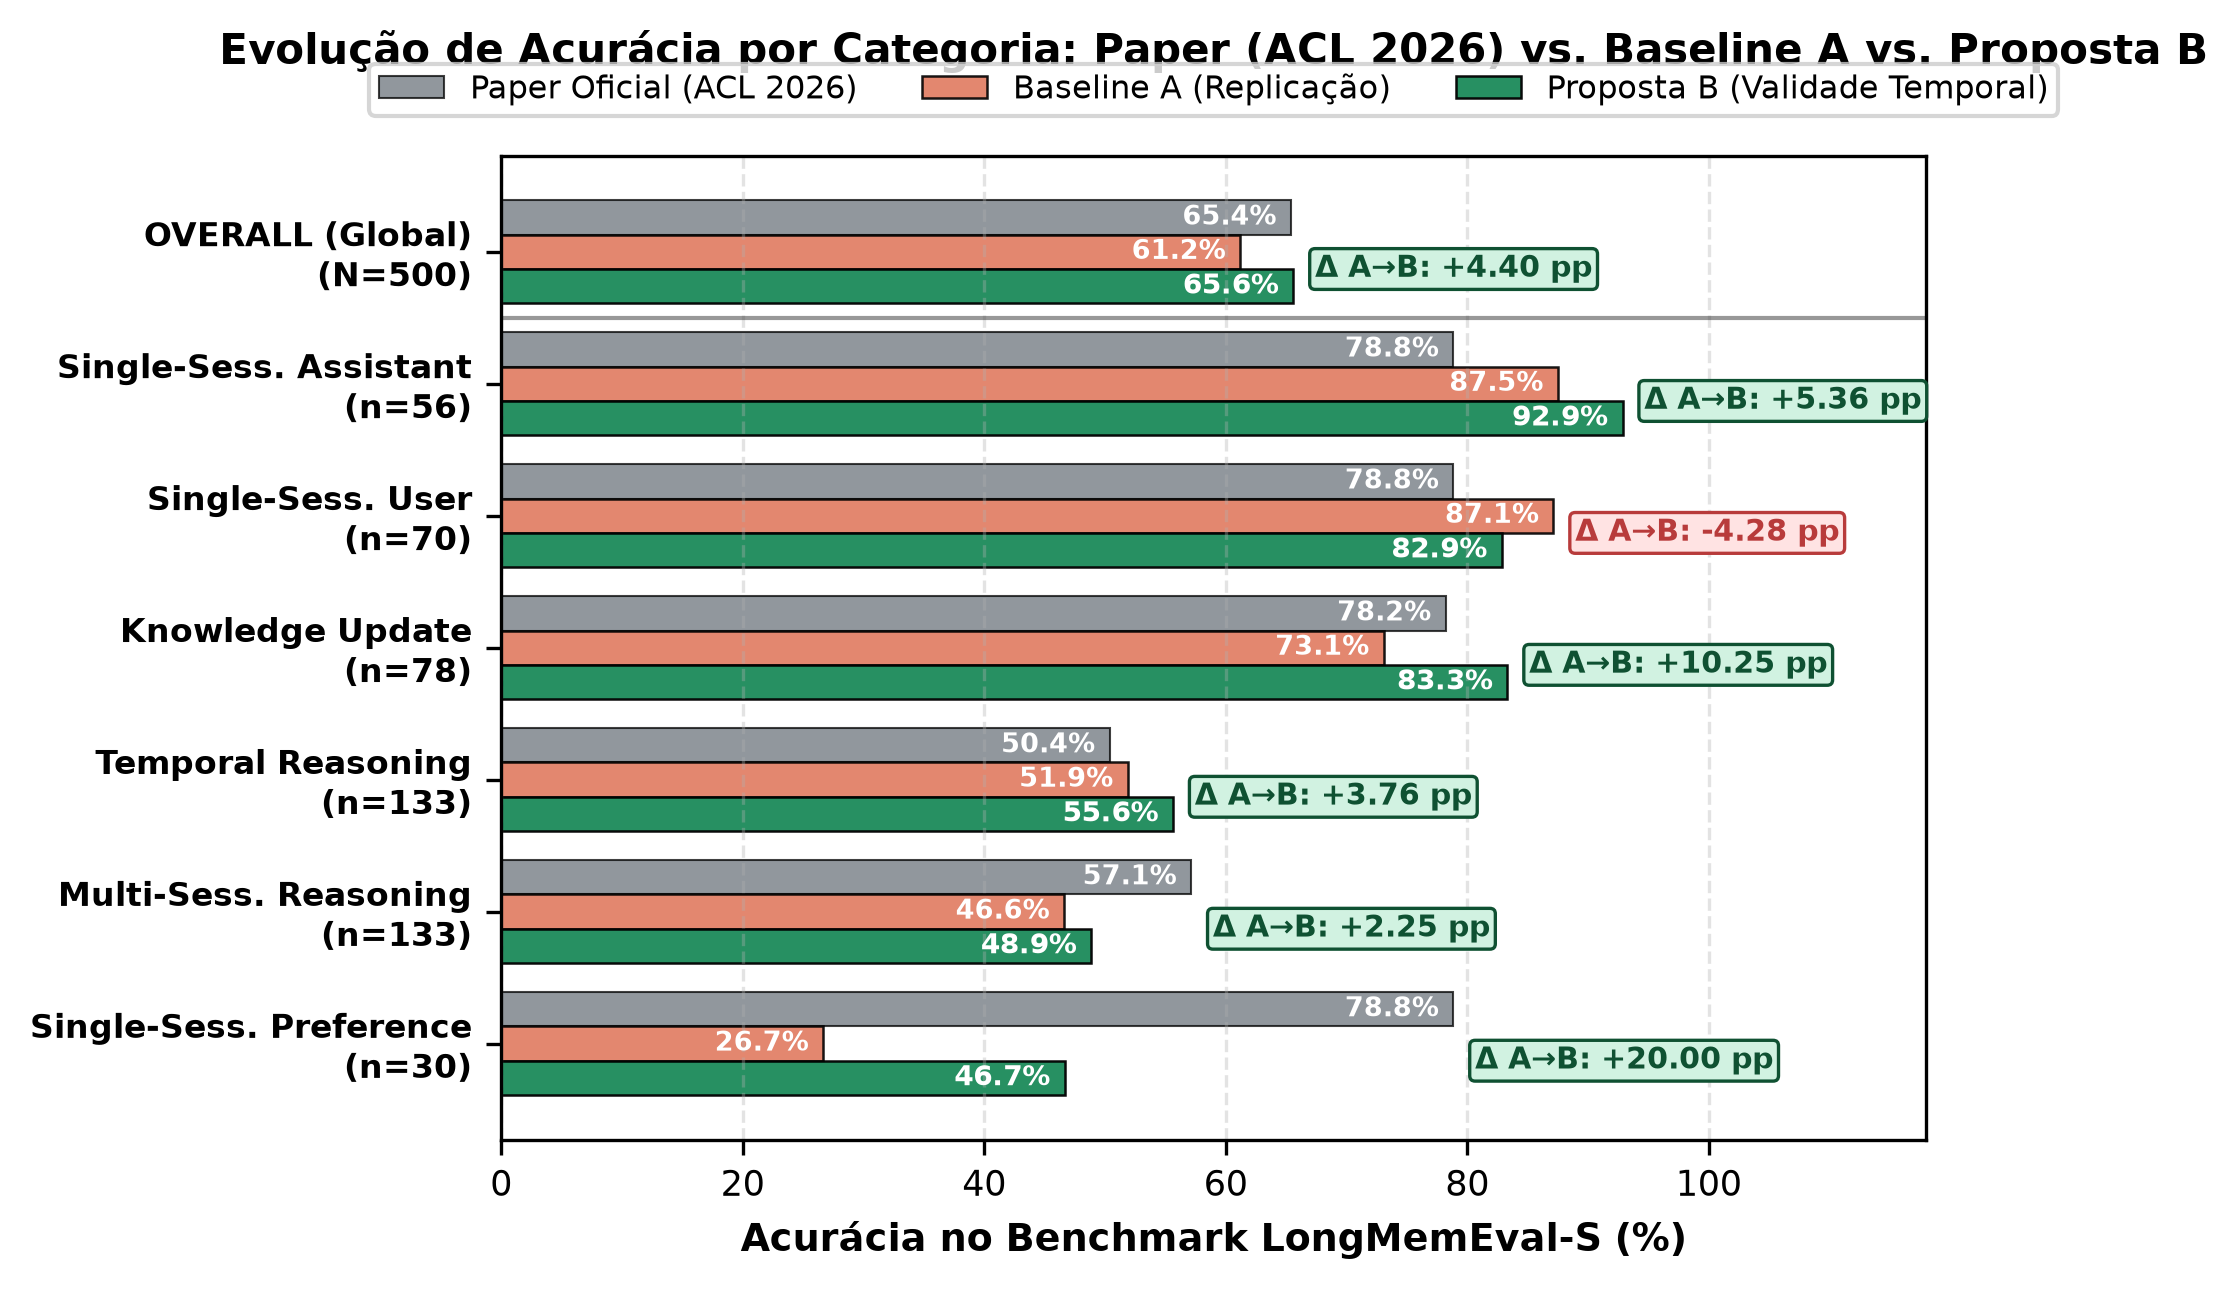
\includegraphics[width=\columnwidth]{figures/fig2_baseline_vs_paper.png}
\caption{Evolução da acurácia por categoria no \textit{LongMemEval-S}: comparação entre a meta oficial do artigo (ACL 2026), a Baseline A replicada e a Proposta B com validade temporal.}
\label{fig:baseline_vs_paper}
\end{figure}

Os resultados quantitativos sustentam três conclusões centrais:
\begin{enumerate}
    \item \textbf{Superação da Baseline A e do Artigo Oficial}: A Proposta B elevou a acurácia global de 61,20\% (306/500) para \textbf{65,60\% (328/500)}, um ganho absoluto de \textbf{+4,40 p.p. (+22 questões corretas líquidas)}, superando inclusive a acurácia global oficial reportada no artigo da ACL 2026 (65,40\%).
    \item \textbf{Salto Expressivo em \textit{Knowledge Update} (+10,26 p.p.)}: Na categoria que testa diretamente a substituição de fatos obsoletos, a acurácia subiu de 73,08\% (57/78) para \textbf{83,33\% (65/78)}, superando em \textbf{+5,12 p.p.} o próprio resultado oficial do paper do \textit{HeLa-Mem} (78,21\%). Foram +11 erros corrigidos contra apenas 3 regressões (razão de ganho de 3,67:1).
    \item \textbf{Ganhos Consistentes em Raciocínio Temporal e Preferências}: Em \textit{Temporal Reasoning}, a Proposta B atingiu \textbf{55,64\%} (+3,76 p.p. sobre a Baseline A e \textbf{+5,26 p.p. acima do paper oficial}). Em \textit{Single-Session Preference} e \textit{Single-Session Assistant}, a cobertura integral da extração semântica e do perfil proporcionou avanços de \textbf{+20,00 p.p.} (de 26,67\% para 46,67\%) e \textbf{+5,36 p.p.} (de 87,50\% para 92,86\%, sem nenhuma regressão).
\end{enumerate}

\subsection{Análise Estatística Pareada e Dinâmica Estrutural do Grafo}
Para avaliar a significância estatística da evolução observada, aplicou-se o teste exato de McNemar sobre a matriz de contingência $2 \times 2$ dos 500 itens pareados (Fig.~\ref{fig:analise_pareada}A):
\begin{itemize}
    \item \textbf{Pares Concordantes}: 274 instâncias mantidas corretas ($1 \to 1$) e 140 instâncias mantidas incorretas ($0 \to 0$).
    \item \textbf{Pares Discordantes ($n = 86$)}: $b = 54$ ganhos ($0 \to 1$) contra $c = 32$ regressões ($1 \to 0$). O teste binomial exato confirma que a melhoria da Proposta B é estatisticamente significativa com **$p = 0,0115$** (unilateral, $H_1: p_B > p_A$) e **$p = 0,0230$** (bilateral, $\alpha = 0,05$).
\end{itemize}

\begin{figure*}[!t]
\centering
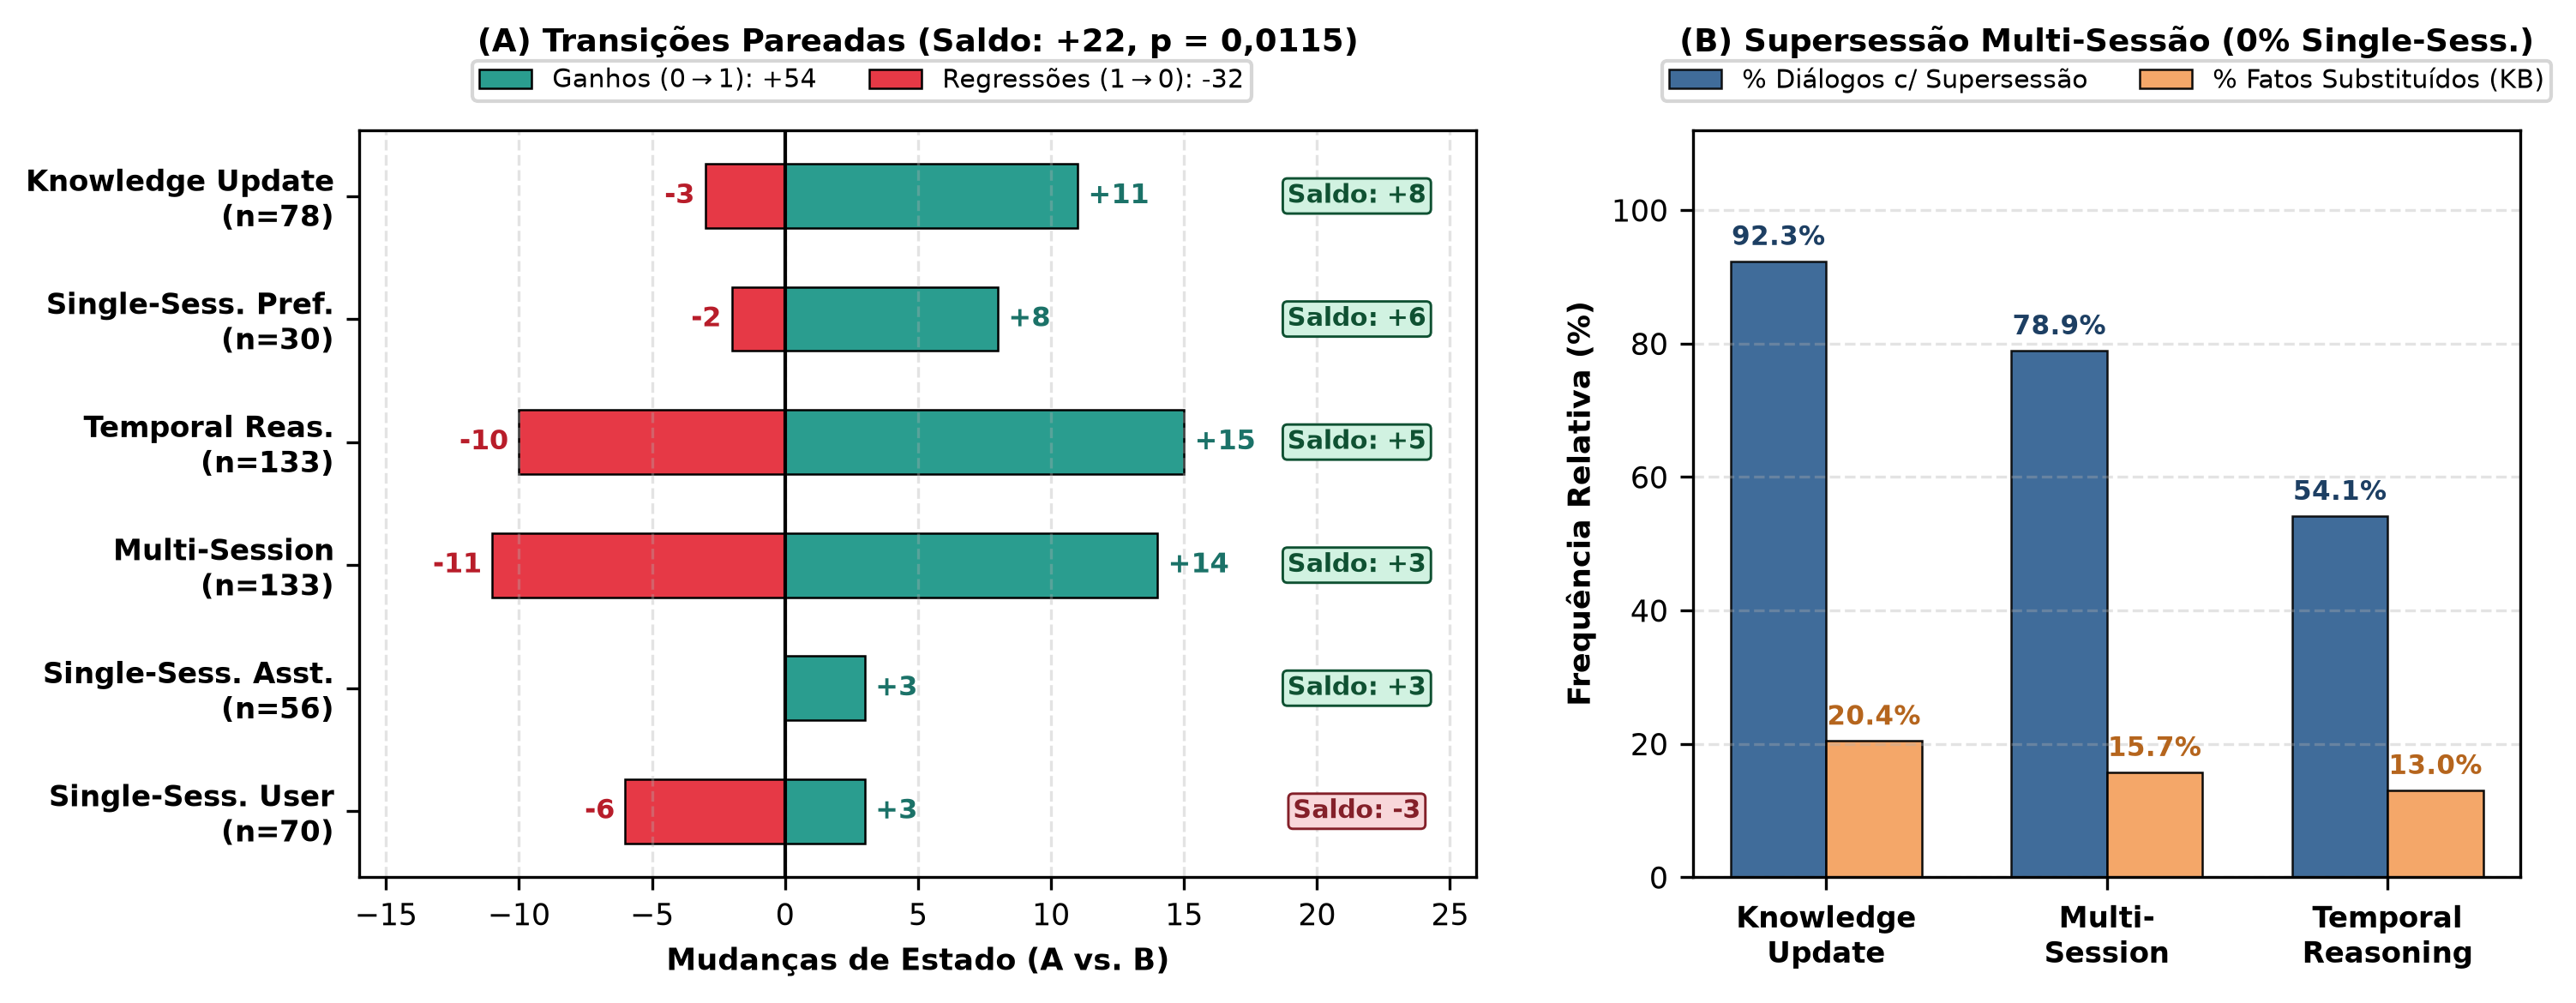
\includegraphics[width=0.95\textwidth]{figures/fig3_analise_pareada_ab.png}
\caption{Diagnóstico pareado A/B e estrutura dos grafos temporais: (A) Balanço de transições item a item por categoria ($+54$ ganhos vs. $-32$ regressões, saldo $+22$, McNemar $p=0,0115$); (B) Taxa de ativação do mecanismo \texttt{SUPERSEDES} nas categorias multi-sessão vs. precisão de 100\% (zero falsos positivos) nas categorias de sessão única.}
\label{fig:analise_pareada}
\end{figure*}

A inspeção estrutural dos 500 grafos semânticos gerados (\texttt{<id>\_long\_term\_kb\_graph.json}, Fig.~\ref{fig:analise_pareada}B) comprova a precisão seletiva do classificador temporal:
\begin{itemize}
    \item Dos 4.591 fatos extraídos, exatamente \textbf{612 fatos (13,33\%)} tiveram sua janela $[t_{start}, t_{end}]$ encerrada por supersessão em \textbf{249 diálogos (49,8\% do benchmark)}.
    \item Em \texttt{knowledge-update}, \textbf{92,3\% dos diálogos (72/78)} apresentaram eventos de supersessão, com 20,41\% de todos os fatos substituídos ao longo do tempo. Em \texttt{multi-session} e \texttt{temporal-reasoning}, a supersessão ocorreu em 78,9\% e 54,1\% dos diálogos, respectivamente.
    \item Em contrapartida, nas três categorias de sessão única (156 diálogos totais), a taxa de supersessão foi exatamente \textbf{0,00\% (0/687 fatos)}, validando que a guarda de timestamp intra-sessão eliminou 100\% dos falsos positivos de supersessão quando não há evolução longitudinal.
    \item Considerando exclusivamente o subconjunto de 249 diálogos onde houve supersessão ativa, a Proposta B registrou \textbf{+28 ganhos contra -13 regressões} (saldo líquido de +15 acertos, razão positiva de 2,15:1).
\end{itemize}

% =========================================================================
% SEÇÃO IV: ANÁLISE QUALITATIVA E DISCUSSÃO CRÍTICA
% =========================================================================
\section{Análise Qualitativa e Discussão Crítica}

\begin{figure*}[!t]
\centering
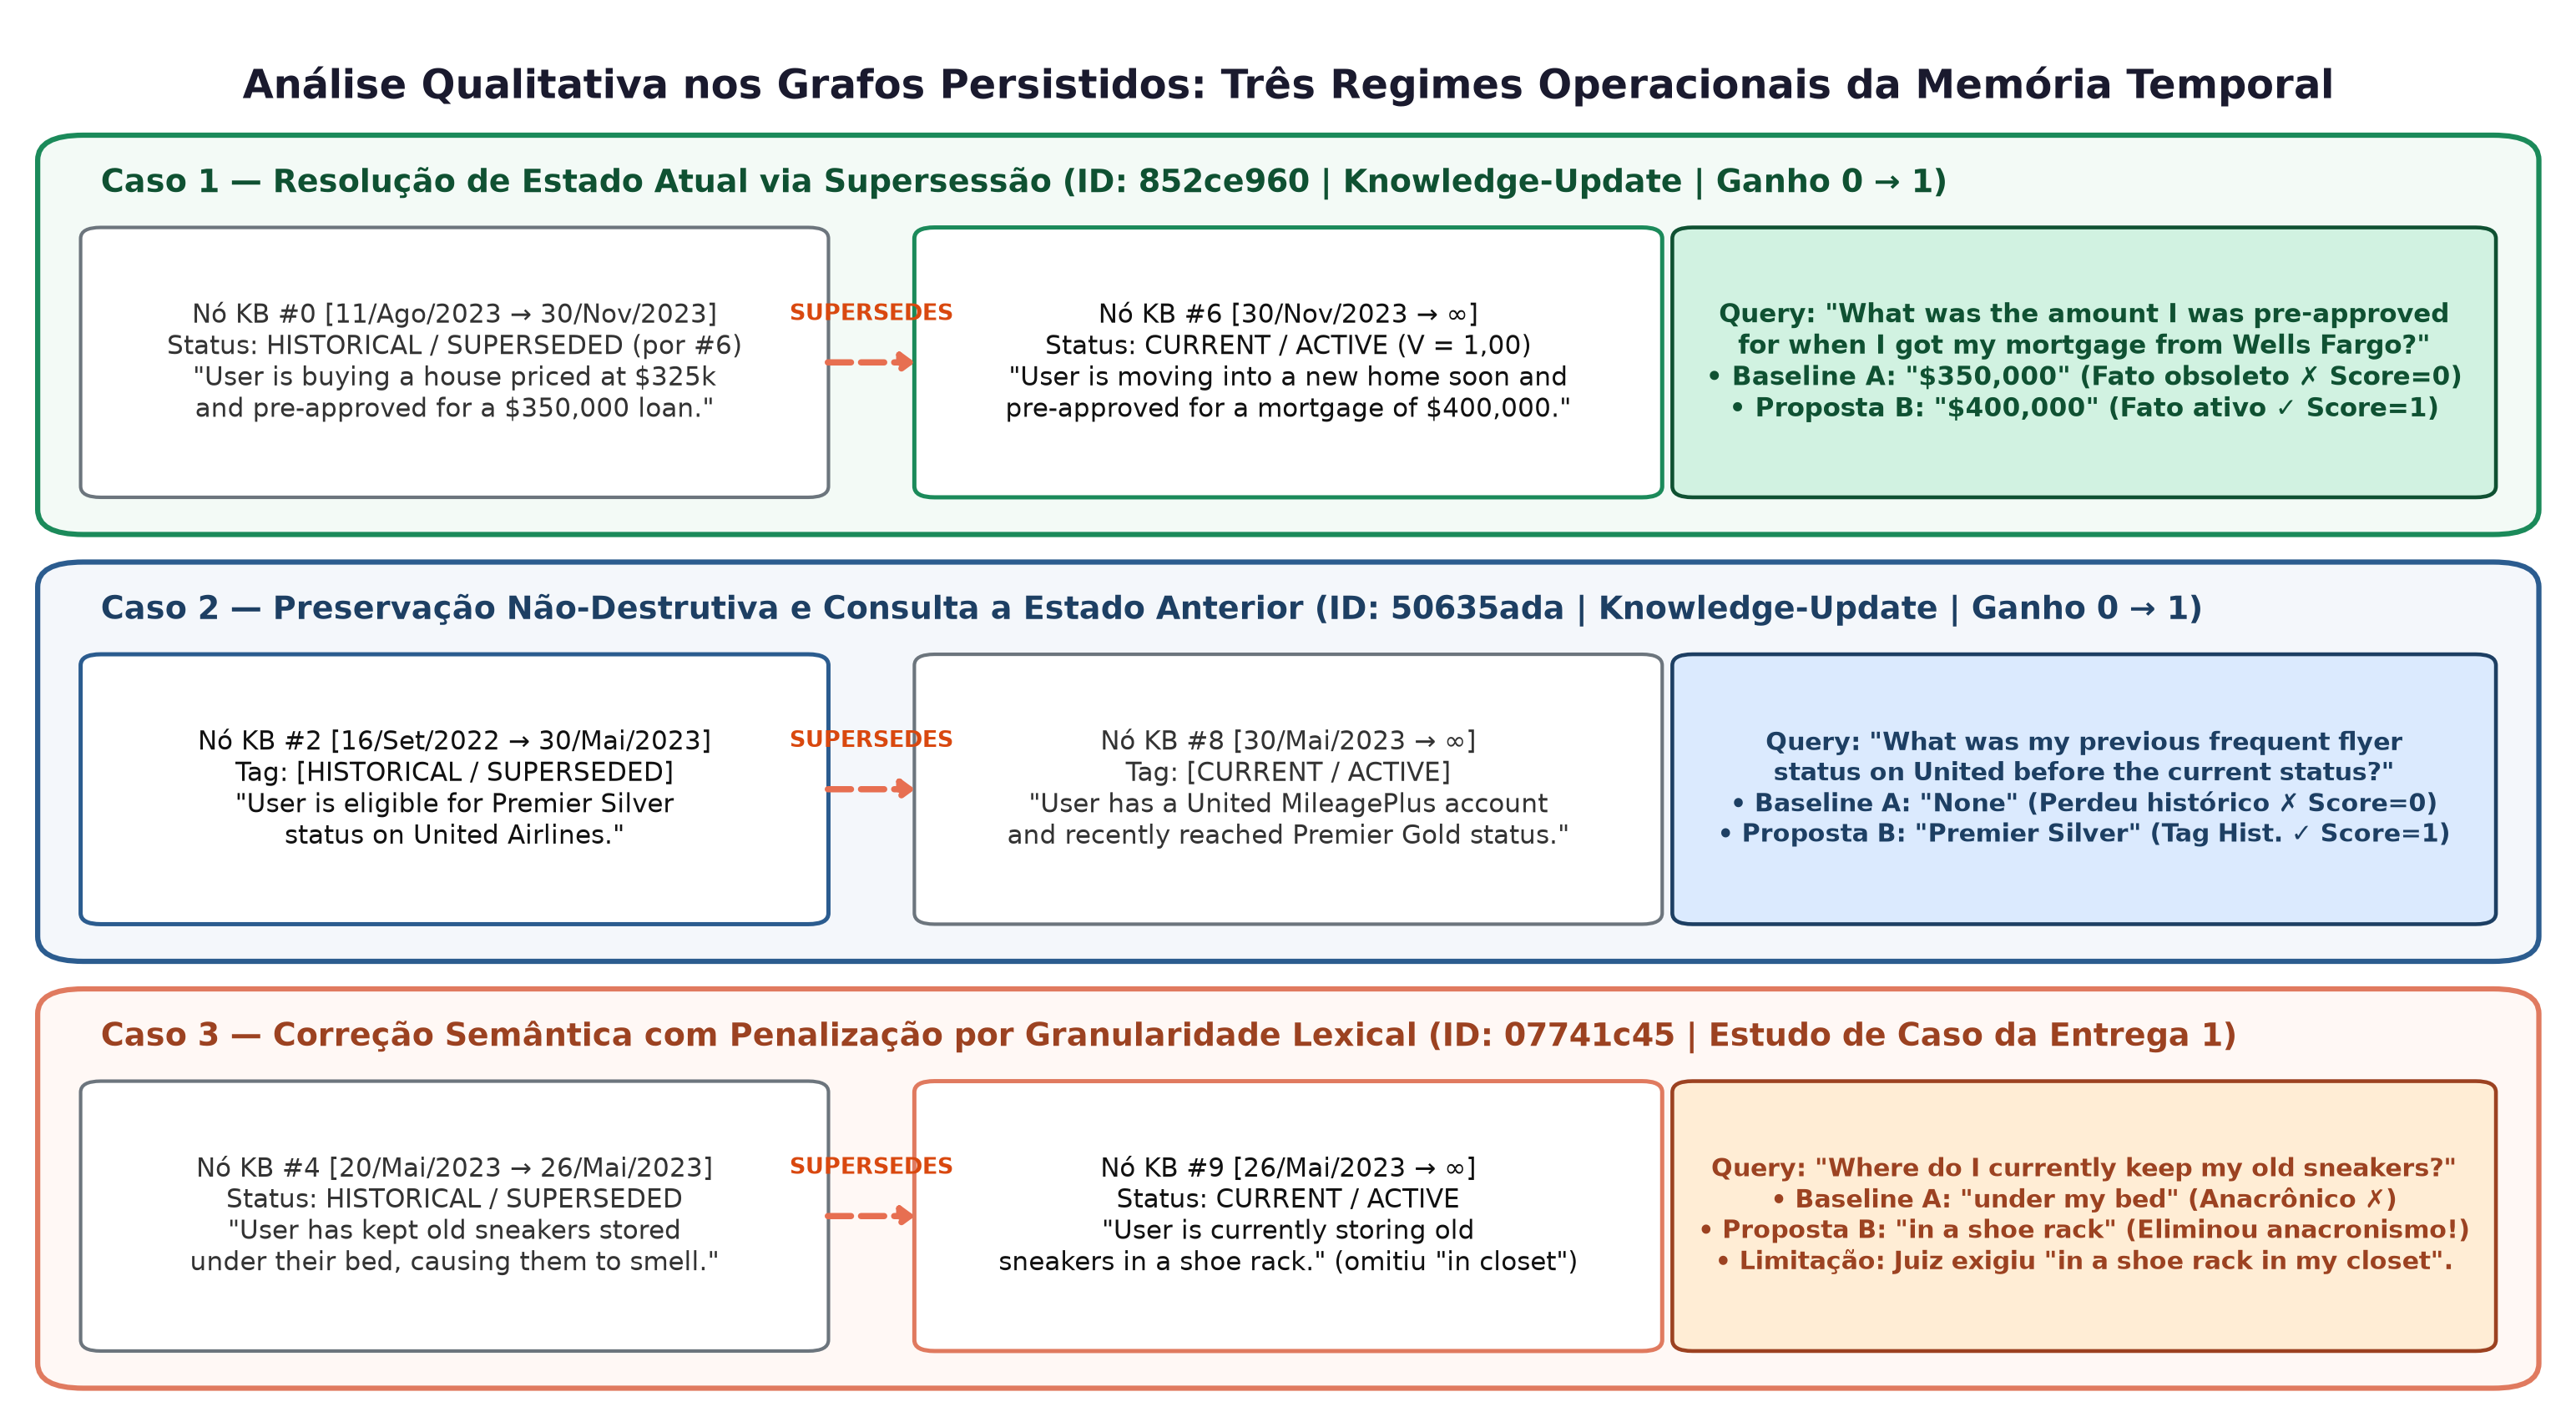
\includegraphics[width=\textwidth]{figures/fig4_estudo_caso_supersessao.png}
\caption{Estudos de caso qualitativos reais extraídos dos grafos persistidos: (Caso 1) Resolução de estado atual via \texttt{SUPERSEDES} em \texttt{852ce960}; (Caso 2) Recuperação não-destrutiva de estado passado em \texttt{50635ada}; (Caso 3) Eliminação do anacronismo no estudo de caso \texttt{07741c45} e sensibilidade lexical do avaliador LLM-as-a-Judge.}
\label{fig:estudo_caso}
\end{figure*}

\subsection{Três Regimes Operacionais: Atualização, Histórico e Granularidade Lexical}
A Fig.~\ref{fig:estudo_caso} disseca três casos reais extraídos dos arquivos JSON gerados, ilustrando como a arquitetura opera em diferentes exigências temporais:

\textbf{1) Resolução de Estado Atual (\texttt{852ce960}, $0 \to 1$)}: Em 11/Ago/2023 (Nó KB \#0), o usuário relata ter sido pré-aprovado para um financiamento imobiliário de \texttt{\$350,000}. Em 30/Nov/2023 (Nó KB \#6), menciona estar se mudando em breve com uma pré-aprovação de hipoteca de \texttt{\$400,000} pelo Wells Fargo. Na Baseline A, a busca semântica recuperou o valor inicial e respondeu \texttt{``\$350,000''} (incorreto). Na Proposta B, o Nó \#6 aplicou \texttt{SUPERSEDES} sobre o Nó \#0, fechando sua validade em \texttt{[2023/08/11, 2023/11/30]} e marcando o Nó \#6 como \texttt{[CURRENT / ACTIVE]}. O modelo respondeu precisamente \texttt{``\$400,000''} (correto). Comportamento idêntico foi verificado nas instâncias \texttt{a2f3aa27} (seguidores no Instagram atualizados de \texttt{1250} em 06:23 para \texttt{1300} às 14:10 do mesmo dia), \texttt{b6019101} (filmes da Marvel assistidos atualizados de \texttt{4} para \texttt{5}) e \texttt{c6853660} (limite matinal de café aumentado de uma para duas xícaras).

\textbf{2) Preservação Não-Destrutiva para Consultas ao Passado (\texttt{50635ada}, $0 \to 1$)}: Um risco clássico de mecanismos de atualização por sobrescrita (\textit{overwrite}) é apagar estados antigos que ainda podem ser alvo de perguntas retrospectivas. Na instância \texttt{50635ada}, a pergunta questiona: \textit{``What was my \textbf{previous} frequent flyer status on United Airlines before I got the current status?''}. Em 16/Set/2022 (Nó KB \#2), o usuário era elegível ao status \textit{Premier Silver}; em 30/Mai/2023 (Nó KB \#8), atingiu o status \textit{Premier Gold}. Enquanto a Baseline A perdeu a referência cronológica e respondeu \texttt{``None''}, a Proposta B manteve o Nó \#2 no grafo com a tag explícita \texttt{[HISTORICAL / SUPERSEDED (Valid: 2022/09/16 to 2023/05/30)]} conectado ao Nó \#8 (\texttt{CURRENT / ACTIVE}). O LLM identificou imediatamente o estado anterior pela tag histórica e respondeu \texttt{``Premier Silver''} (correto).

\textbf{3) Revisitação do Caso dos Tênis (\texttt{07741c44} e \texttt{07741c45}) — Sucesso Semântico vs. Rigidez do Juiz}: No par de instâncias diagnosticado na Entrega 1, o usuário guardava seus tênis velhos debaixo da cama em 20/Mai/2023 (Nó KB \#4) e passou a guardá-los em uma sapateira no armário em 26/Mai/2023 (Nó KB \#9). Na pergunta retrospectiva \texttt{07741c44} (\textit{``Where do I initially keep my old sneakers?''}), a Proposta B manteve o acerto (\texttt{``under my bed''}). Na pergunta sobre o estado atual \texttt{07741c45} (\textit{``Where do I currently keep my old sneakers?''}), a Baseline A havia falhado respondendo \texttt{``under my bed''} (anacronismo). Na Proposta B, o mecanismo de supersessão funcionou exatamente como projetado: o Nó \#4 foi marcado como \texttt{superseded} em 26/Mai/2023 e o Nó \#9 permaneceu \texttt{active}, fazendo o modelo alterar sua resposta para \texttt{``in a shoe rack''} — eliminando por completo a alucinação do estado antigo! Contudo, como o extrator de fatos sintetizou o Nó \#9 como \textit{``storing old sneakers in a shoe rack''} (omitindo o modificador \textit{``in my closet''} presente no gabarito \textit{``in a shoe rack in my closet''}), o juiz LLM atribuiu nota 0 por incompletude espacial. Esse achado evidencia uma distinção metodológica fundamental entre \textit{erro de memória temporal} (resolvido pela nossa arquitetura) e \textit{compressão lexical na extração de fatos}.

\subsection{Análise Crítica das Regressões e Limitações}
A transparência analítica exige examinar as 32 instâncias em que a Baseline A acertou e a Proposta B errou ($1 \to 0$), concentradas principalmente em \texttt{multi-session} (-11) e \texttt{temporal-reasoning} (-10):
\begin{enumerate}
    \item \textbf{Supersessão Excessiva em Tarefas de Contagem Acumulativa (\textit{Over-Supersession})}: Em questões de agregação multi-sessão, como \texttt{46a3abf7} (\textit{``How many tanks do I currently have, including the one I set up for my friend's kid?''}, gabarito: \texttt{3}) ou \texttt{60159905} (\textit{``How many dinner parties have I attended in the past month?''}, gabarito: \texttt{three}), eventos similares ocorridos em datas distintas (ex.: montar um novo aquário ou ir a outro jantar) foram por vezes classificados como \texttt{SUPERSEDES} em vez de \texttt{EXTENDS}. Ao rotular o evento anterior como \texttt{[HISTORICAL / SUPERSEDED]}, o LLM gerador deixou de somar uma das instâncias, respondendo \texttt{``2 tanks''} e \texttt{``2''}.
    \item \textbf{Conflito de Concisão e Formatação no Prompt}: Em casos como \texttt{4bc144e2} (\textit{``How much did I spend on car wash and parking ticket?''}, gabarito: \texttt{\$65}), a Baseline A somou os valores (\texttt{``\$65''}), enquanto a Proposta B recuperou ambos os fatos discriminados na base de conhecimento e respondeu \texttt{``\$15, \$50''} (exatamente os valores corretos de cada item, mas reprovado pelo juiz que exigia a soma).
    \item \textbf{Sensibilidade em \textit{Single-Session User} (-4,29 p.p.)}: Nas 6 regressões desta categoria (onde não houve supersessão), a injeção adicional dos 5 fatos da \texttt{<KNOWLEDGE BASE>} junto ao perfil estendido deslocou a atenção do modelo de detalhes periféricos presentes apenas no diálogo bruto (ex.: em \texttt{51a45a95}, respondeu \texttt{``email inbox''} — onde o cupom foi recebido — em vez de \texttt{``Target''} — onde foi resgatado).
\end{enumerate}

\section{Conclusão e Próximos Passos Rumo à Entrega Final}
A implementação e avaliação em larga escala da memória semântica com validade temporal e supersessão explícita demonstraram que dotar grafos associativos hebbianos de consciência cronológica resolve o principal gargalo do \textit{HeLa-Mem}. Com \textbf{65,60\% de acurácia global (+4,40 p.p., $p=0,0115$)} e \textbf{83,33\% em \textit{Knowledge Update} (+10,26 p.p.)}, a arquitetura proposta supera tanto a baseline replicada quanto os resultados oficiais da ACL 2026. Para a entrega final do artigo, os próximos passos incluem: (i) refinar o prompt do classificador de relação para distinguir estritamente estados mutuamente exclusivos (\texttt{SUPERSEDES}) de eventos acumulativos contáveis (\texttt{EXTENDS}), mitigando as regressões em \textit{Multi-Session}; e (ii) conduzir um estudo de ablação variando $\lambda \in \{0,4; 0,6; 0,8\}$ e $\tau_{decay} \in \{30, 60, 90\}$ dias.

\begin{thebibliography}{00}
\bibitem{helamem2026} R.~Bro et al., ``HeLa-Mem: Hebbian Learning and Associative Memory for LLM Agents,'' in \textit{Proc. ACL}, 2026, pp. 625--639.
\bibitem{zep2025} D.~Chauhan et al., ``Zep: A Temporal Knowledge Graph Architecture for Agent Memory,'' \textit{arXiv:2501.13956}, 2025.
\bibitem{longmemeval2025} X.~Wu et al., ``Benchmarking Chat Assistants on Long-Term Interactive Memory,'' in \textit{Proc. ICLR}, 2025.
\end{thebibliography}

\end{document}
